\documentclass{article}
\usepackage[a4paper, textwidth=14cm]{geometry}
\usepackage{graphicx} % Required for inserting images

\usepackage{hyperref}
\usepackage{cleveref}
\usepackage{listings}
\usepackage{ mathrsfs }

\title{\textbf{Controllable Music Generation}}
\author{Michael Büttner \and Johanna Pries \and David Komnick}
\date{\vspace{-3ex}}
\graphicspath{ {./images/} }
\usepackage{subcaption} 


\begin{document}

\maketitle

\section{Introduction}
Music is an important topic for most people in their day-to-day life and we are constantly surrounded by it. But composing music is a very complex art which requires a lot of knowledge. So in addition to human compositions, which are made by hand, there is also the approach to generate music via algorithms. For this to be well functioning it is critical to make the music generation controllable. In general, it would be practical if not the user would have to choose which music they want to listen to, but the music would be automatically chosen based on the mood etc. the user is in at the moment.
Our idea is to generate music depending on the the mood a person is currently in. 


\section{Methods}
The general idea was to work with successful and promising, already published related work (and file formats) and expand, adapt and improve those approaches for our needs and goals. A substantial part of our work was the modification of FIGARO (FIne-grained music Generation via Attention based, RObust control).

\subsection{MIDI}
The MIDI (Musical Instrument Digital Interface) data file format has become a widely adopted standard in the music industry due to its flexibility, efficiency, and controllability. Unlike WAV (Waveform Audio File Format), which represents audio waveforms as raw sampled data, MIDI files store musical information in a symbolic format that encompasses note events, timing, pitch, duration, and other relevant musical parameters. This symbolic representation makes MIDI files highly suitable for controllable music generation with AI.

We decided to use the MIDI data file format instead of the WAV format, because of its inherent advantages in controllable music generation with AI. Another advantage of the MIDI file format is that it is extendable to other formats, such as the the REMI (REvamped MIDI-derived events) \cite{DBLP:journals/corr/abs-2002-00212} and REMI+ \cite{von2022figaro} file format.

\subsection{REMI}
REMI was introduced to represent MIDI data following the way humans read them. In addition to the tokens used in the MIDI file format, REMI uses 'Bar' and 'Position' events, indicating the beginning of a bar and the specific position within a bar (quantized to 16 regions), respectively. This structure leads to better rhythmic regularity when modeling music and replaces the need of using a 'Time-Shift' event. In comparison to MIDI, a set of 'Tempo' events was added to REMI to allow for local tempo changes per beat. Additionally, a 'Chord' event was added to make the harmonic structure of music explicit and therefore improve controllability of the chord progression. A chord consists of a root note (C, C\#, D, ...) and a chord quality (major, minor, diminished, ...). Other than in the MIDI format, REMI does not use 'Note-Off' events, but instead uses 'Note Duration' events. Hence, each note is represented with the 'Note Velocity', 'Note-On' and 'Note Duration' event. This gives the advantage, that the duration of a note does not have to be inferred from a time gap and a model does not have to learn that 'Note-On' and 'Note-Off' events must appear in pairs \cite{DBLP:journals/corr/abs-2002-00212}.

\subsection{REMI+}
The original REMI format does not allow for modeling multiple tracks or multiple time signatures. Therefore, REMI+ was introduced as an extension to REMI. REMI+ is suitable for general multi-track, multi-signature symbolic music sequences. This is done by modifications that add time signature and instrument information, determining a unique order of events and use quantization schemes that allow an accurate representation for a diverse set of music \cite{von2022figaro}.

\subsection{FIGARO}
We are using a transformer model for music generation called FIGARO \cite{von2022figaro}. It uses a self-supervised description-to-sequence task to generate symbolic music. There are two kinds of descriptions the model can take as an input. The first one is the expert description (\cref{fig:Figaro}), which includes certain features per bar, such as time signature, note density, mean pitch, mean velocity, mean duration, instruments and chords. It serves as a human interpretable feature description but is only able to capture low-fidelity features.  

The other possible input type is the learned description. It is gained through the use of a Vector Quantized Variational Autoencoder (VQ-VAE) framework. The framework is trained separately to FIGARO and the latent code is used as the learned description. 

The main part of FIGARO is a sequence-to-sequence model which takes either the expert description, the learned description or both as an input and gives music as an output.
The authors of FIGARO proposed and used the REMI+ format. Because of this, we have to convert all inputs from MIDI to REMI+ and all outputs from REMI+ to MIDI. 

As shown in Figure \ref{fig:Figaro}, FIGARO is build out of two transformers using an encoder-decoder architecture. In the forward-path of FIGARO the hidden state is passed from the encoder to the decoder.

\begin{figure}[h]
\centering
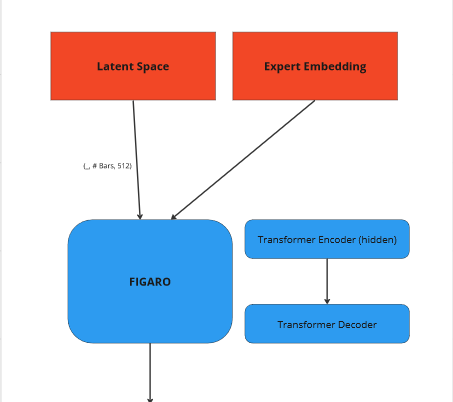
\includegraphics[width=8cm]{Figaro}
\caption{Encoder-decoder architecture of FIGARO (blue) and latent space and expert embedding as input (red).}
\label{fig:Figaro}
\end{figure}

The encoder from FIGARO is processing a varying context size of input tokens into a latent representation. The input has a shape of $(\#\texttt{batches}, \texttt{n-tokens})$ and it is processing it into $(\#\textbf{batches}, \texttt{context-size}, \texttt{n-tokens})$ where 
$\texttt{n-token}=1357$ is the number of tokens. Output of the encoder is used as hidden space for the decoder.

The decoder from FIGARO takes 2 inputs: The hidden space from the encoder and the known tokens. Let the "known tokens" be $x$ with the shape $(\#\texttt{batches}, \#\texttt{tokens})$. The output shape is defined by $x$, the output $z$ have a shape of $(\#\texttt{batches}, \#\texttt{tokens}, \texttt{n-tokens})$. We can get the token-ids by applying $\texttt{armax}$ over the tokens. Comparing $x$ and $y$, all tokens from $x$ are shifted one to the left. We drop the first token and add a new generated last token. Most tokens did not change and were only shifted, some changed slightly.

\subsection{Datasets}
In order to train the emotion-classifier, an appropriate dataset is needed. We decided to use the EMOPIA dataset \cite{{EMOPIA}} for this process. EMOPIA is a database including MIDI data which focuses on perceived emotion in pop piano music. The dataset contains 1,087 music clips annotated with emotion labels by hand. In the dataset the perceived emotions are divided into four quadrants (Q1, Q2, Q3, Q4). These quadrants are defined by the level of valence and the level of arousal (low or high respectively) in the music (see Table \ref{tab:emopia_valence_arousal}). The number of clips and the average length of the music clips in each quadrant slightly differ from each other (see Table \ref{tab:emopia_quadrants_clips}). Quadrant Q4 contains 50 to 60 music clips more than the other three quadrants. Those quadrants only vary a little bit in their number of clips. Quadrant Q3 has the highest average length in seconds and Q2 has the highest average length measured in number of tokens.
We used all four quadrants for the training. The quadrants which differ the most from each other are Q1 and Q3. These differences can be perceived by hearing but are also shown in regard of note density, note length and note velocity. For quadrant Q1 the corresponding music is perceived as exciting. The music in quadrant Q3 is perceived as calm. Therefore, those two quadrants are suitable for comparing and perceiving their differences in the generated results.

\begin{table}[]
\centering
\caption{The four different quadrants of the EMOPIA dataset divided by the level of valence and arousal in the contained music clips.}
\label{tab:emopia_valence_arousal}
\begin{tabular}{|l|l|l|}
\hline
             & Low valence & High valence \\ \hline
High arousal & Q2          & Q1           \\ \hline
Low arousal  & Q3          & Q4           \\ \hline
\end{tabular}
\end{table}

\begin{table}[]
\centering
\caption{The four different quadrants of the EMOPIA dataset with their respective number of contained music clips and the average length of those clips measured in seconds and in number of tokens.}
\label{tab:emopia_quadrants_clips}
\begin{tabular}{|l|l|l|l|}
\hline
Quadrant & \#clips & Avg. length (in sec) & Avg. length (in \#tokens) \\ \hline
Q1       & 250     & 31.9                 & 1,065                     \\ \hline
Q2       & 265     & 35.6                 & 1,368                     \\ \hline
Q3       & 253     & 40.6                 & 771                       \\ \hline
Q4       & 310     & 38.2                 & 729                       \\ \hline
\end{tabular}
\end{table}

\subsection{Classifier}
Together with the EMOPIA dataset, several emotion classifiers were introduced and evaluated. The classification task for EMOPIA was defined as classifying a song into one of the four categories (quadrants) described in the section above. For this, the classification results were obtained on symbolic-domain emotion recognition as well as on audio-domain emotion recognition. The symbolic-domain classification includes using two different symbolic note representation methods: MIDI-like and REMI \cite{{EMOPIA}}. For our purposes the symbolic-domain classifier utilizing the REMI input files is suited. 

The model is build as a combination of a bidirectional LSTM and a self-attention module. The temporal information of the songs is extracted by the LSTM. The self-attention module on the other hand computes weight vectors over the hidden states of the LSTM with multi-head attention. Eventually, the resulting weighted hidden states are used for the classification \cite{{EMOPIA}}.

For our work this classifier can be repurposed but it first has to be adapted to REMI+.

\section{Experiments}
In order to use FIGARO for our purposes, several parts of the model had to be adapted and extended.

\subsection{Changing the FIGARO expert description}
Since the expert description includes the chords per bar, one first naive idea is to change all the chords to their relative minor or relative major to manipulate the perceived emotion. For example a 'C Major' chord would be rewritten as an 'A Minor' chord and vice versa. This way the musical relations between different chords are conserved in contrast to simply changing the chords to their parallel key (i.e. from major to minor, or the other way around), without adapting the tonic note. But still several other problems are encountered. It is for instance unclear what happens with augmented our diminished chords as those types of chords can be assigned to neither major nor minor scales.

This approach was not further pursued in the project.

\subsection{Sampling from the FIGARO latent space}
Another approach is to sample music directly from the FIGARO latent space. For this we need a method to generate hidden samples in the latent space based on the emotion labels. The decoder from FIGARO is turning these generated hidden samples into music, represented in the REMI+ file format. Since we use a pretrained FIGARO model, we only have to provide good hidden spaces based on an emotion label. We train a Conditional Variational Autoencoder (CVAE) for compressing the hidden samples into a low-dimensional standard normal distribution with a condition label. For generating music we can sample from the hidden space of the CVAE. By this we get music.

\subsubsection{Training}
We want to train a \textit{cVAE} generating a hidden state for the decoder of FIGARO. We condition the \textit{cVAE} on the emotion label of the music. By this we want to be able to generate hidden states for FIGARO of a specified emotion.

Let $X$ be the set of possible data points, $\mathscr{L}$ the low-dimensional latent space and $C$ the finite set of possible class labels. We train the \textit{cVAE} on a labeled finite data set $S \subset (X \times C)$. A \textit{cVAE} is build of an encoder $e: X \rightarrow \mathscr L$ and a decoder $d: C \times \mathscr L \rightarrow X$. By giving the decoder the information of the class label, we want to achieve that the class information is not encoded in the latent space. As our training objective we want to have $d(e(x), c) = x$ and we want our distribution of the latent space to be normal distributed.

As loss function we take a combination of the huber-loss and the loss resulting from the Kullback-Leibler divergence. We train our \textit{cVAE} for 20 epochs.

We did not condition that each label shell be represented normal-distributed. Even though it is crucial for the sampling process from the latent space to assume that each label in normal distributed. We can test our assumption by observing the average mean and the average log variance for each (emotion) label.

\begin{figure*}[ht!]
    \subcaptionbox{}{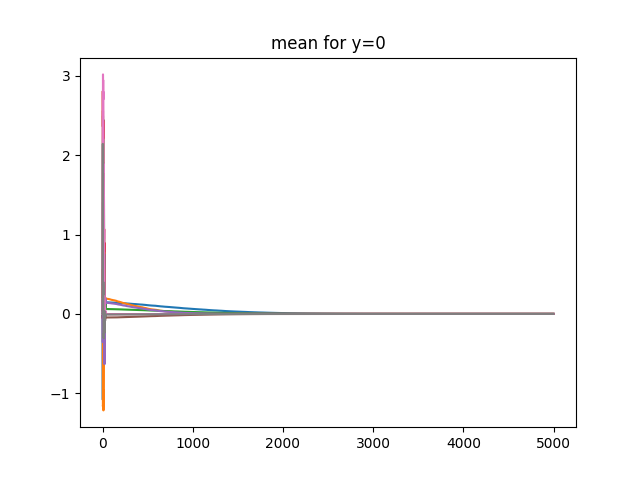
\includegraphics[width=0.45\textwidth]{images/mean_y0.png}}
    \hfill
    \subcaptionbox{}{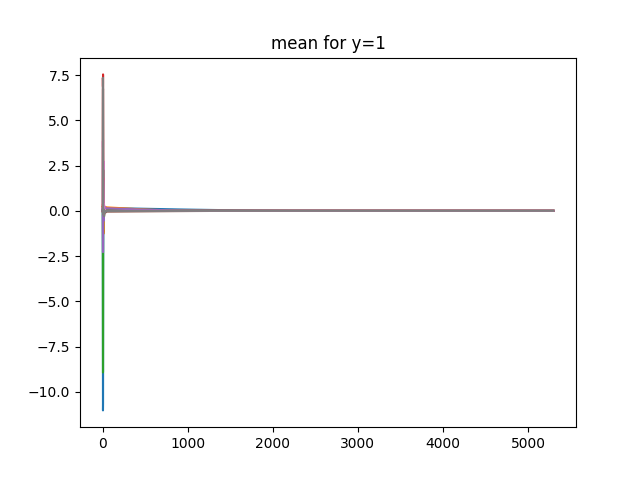
\includegraphics[width=0.45\textwidth]{images/mean_y1.png}}
    \subcaptionbox{}{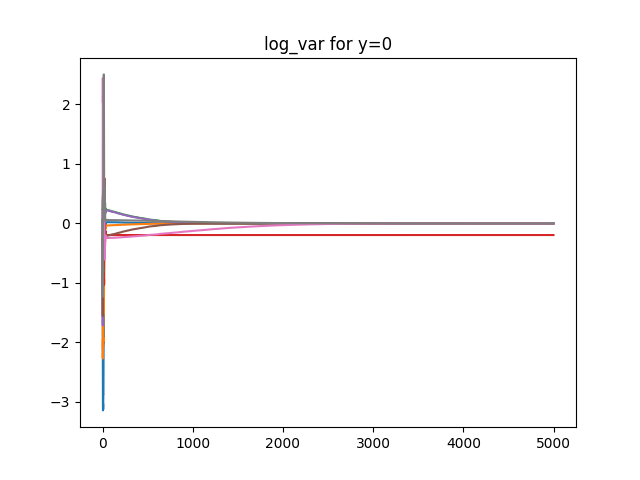
\includegraphics[width=0.45\textwidth]{images/log_var_y0.png}}
    \hfill
    \subcaptionbox{}{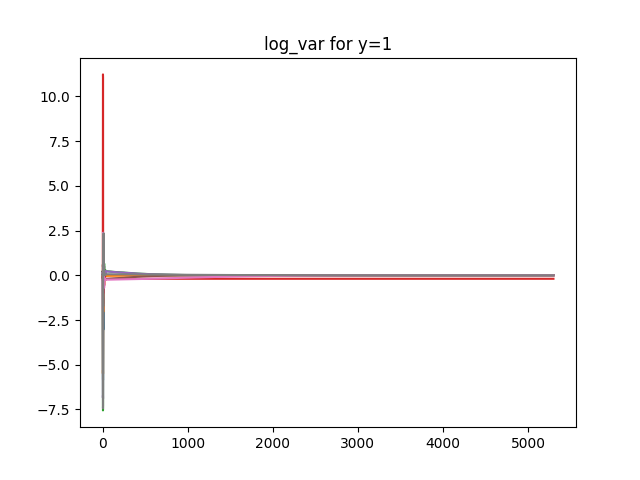
\includegraphics[width=0.45\textwidth]{images/log_var_y1.png}}
    \caption{average mean and log-var plotted for the class labels 1 and 2}
    \label{fig:means}
\end{figure*}

We can see in figure \ref{fig:means} we can see that the assumption holds, that the mean and logarithmic variance is close to 0. Now we know, that we can sample from the latent space and condition on emotions. We can expect the hidden space to be meaningful.


\subsubsection{Loss function}
The loss function used for training the CVAE is a combination of the Huber loss and the Kullback-Leibler divergence (KLD). The Huber loss is used because it is less sensitive to outliers in data than the squared error loss. As a reduction method for the Huber loss, we used the mean, which leads the sum of the output to be divided by the number of elements in the output. The KLD measures the divergence between one probability distribution and a reference probability distribution (standard normal distribution). Adding the Huber loss to the KLD yields our loss function.


\section{Results}
In order to state our results we will look into the measurable outcomes of our generation, but we will also describe our impressions on the generated music.

Our classifier has a validation accuracy of 0.704 for all 4 quadrants, which is comparable to the accuracy achieved by \cite{EMOPIA}, and and accuracy of 0.969 for the quadrants Q1 and Q3. 

In all of our approaches the outcomes are similar. The classifier labels most songs as quadrant Q1 (high arousal, high valence) and some songs as Q2 (high arousal, low valence), no matter which class label we give to the CVAE. The other two quadrants are not represented in the classification results. While listening to the songs ourselves we would also classify most songs as high arousal, high valence, although there are sections of some songs we perceived as rather calm. In general it is difficult to notice differences between the generated music of the various classes. 

It is interesting to note that the instruments used in the songs vary, although the CVAE is trained on only piano pieces. The choice of instruments in a song is relatively consistent when we generate one hidden state per song. If we generate a new hidden state every bar, new instruments appear each bar and are not consistently used throughout the song.

The quality of the songs is rather desirable and cannot be compared with music composed by humans. There are parts of the music that sound coherent and rhythmical but those parts often last only a few bars and are then again replaced by unmelodic parts. Furthermore, there are many sudden tempo shifts during the songs. When using the same seed but with different emotion labels, we notice that the instruments across the songs are similar, but the melodies are vastly different. We did not notice any consistent differences across these songs regarding valence or arousal. Some music we generated had parts in it which were silent. We did not observe this in the music that was reconstructed by FIGARO.

Generally, we find that using the \textit{figaro-learned} model for dataset generation and music generation yields better results compared to using the combined \textit{figaro} model, as it has more consistent parts inside its songs. 

\section{Discussion}
We must keep in mind that we cannot expect perfectly generated music: Parts from the reconstructed music by FIGARO from the example code is not melodic and arhythmic. We take it as an upper bound for the quality we can expect of the generated music. Another possible reason for failure is the large size of the FIGARO hidden state. We compress a vector of the size 131,072 into a latent space with the size 8, and due to computational reasons, we can not make our model too big. A compression by this amount may lead to inaccuracies.

\subsection{Future Work}
Our work does not have to be limited on emotion related tasks. It could be adapted to several other domains. Instead of a dataset classified based on emotion, for example a dataset divided into different genres of music could be used. This way the output would not be restricted to different emotions conveyed in the music, but could provide, for example, different types of music. Depending on changes detected in the environment, classical, pop, rock, metal or country music could be generated. This is just one of many possibilities how our work could be expanded.

Generally, to improve the results, music clips with different kinds of complexities could be chosen. It could be potentially beneficial to use simple and not too complex music clips to improve the quality of the generated music.

\subsection{Conclusion}
We suggest a new approach to music generation which is to create music based on a certain emotion label. We use the existing FIGARO model for controllable music generation. To guide the generation process with emotion labels, we train a separate conditional VAE that is conditioned on them. We take the decoder from the trained CVAE to generate a latent representation from an emotion label and random samples, which is then passed to FIGARO to produce the final piece. The result of this system is promising, while FIGARO generates fluent and coherent music, the CVAE ensures that the music follows a pattern that indicates a certain emotion consistently.


\bibliographystyle{ieeetr}
\bibliography{citation} 

\end{document}